\section{Background: Goal-oriented Requirements Language and argument schemes}
\label{sect:background}

In this section, we first introduce our running example, after which we introduce the Goal-oriented Requirements Language (GRL)~\cite{Amyot:2010:EGM:1841349.1841356}, which is the goal modeling language we use to integrate with the argumentation framework. Next, we introduce argument schemes, and in particular, we discuss the \emph{practical reasoning argument scheme (PRAS)}~\cite{atkinson2007}, which is an argument scheme that is used to form arguments and counter-arguments about situations involving goals. Finally, we give an overview of the integration between PRAS and GRL.  %This will be our starting point in the next section.

\subsection{Running example: Traffic Simulator}
\label{sect:goals:runningexample}

We use the traffic simulator design case to explain the concepts and the framework in this paper. Traffic simulator design is the topic of discussion in the transcripts used for argumentation framework.   
%Most of the examples in this article, as well as the topic of discussion in the transcripts we analyze, come from the traffic simulator design exercise. 
In this exercise, designers are provided with a problem description, requirements, and a description of the desired outcomes. The problem description is given in full in Appendix~\ref{sect:designprompt}, and is summarized as follows: The client of the project is Professor E, who teaches civil engineering courses at an American university. In order for the professor to teach students how various theories (such as queuing theory) around traffic lights work, a software analyst is hired to specify the goal and requirements of the system. %and It is the task of the designer to specify a system in which the professor can teach students how various theories around traffic lights works, such as queuing theory. 
To this end, a piece of software will be developed in which students can create visual maps of an area, regulate traffic, and so forth. The original version of the problem descrption~\cite{UCIworkshop} is well known in the field of design reasoning and it has been used in a workshop\footnote{\url{http://www.ics.uci.edu/design-workshop/}}. Transcripts of this workshop have been analyzed in detail~\cite{Petre:2013:SDA:2535028}. Although the concepts of traffic lights, lanes, and intersections are common and appear to be simple, building a traffic simulator to represent these relationships and events in real time turns out to be challenging.

\subsection{Goal-oriented Requirements Language (GRL)}
\label{sect:background:grl}
GRL is a visual modeling language for specifying intentions, business goals, and \emph{non-functional requirements} of multiple stakeholders \cite{Amyot:2010:EGM:1841349.1841356}. GRL is part of the User Requirements Notation, an ITU-T standard, that combines goals and non-functional requirements with functional and operational requirements (i.e. use case maps) in one. GRL can be used to specify alternatives that have to be considered, decisions that have been made, and rationales for making decisions. A GRL model is a connected graph of intentional elements that optionally are part of the actors. All the elements and relationships used in GRL are shown in Figure~\ref{fig:grl_legend}.

\begin{figure}[ht]
\centering
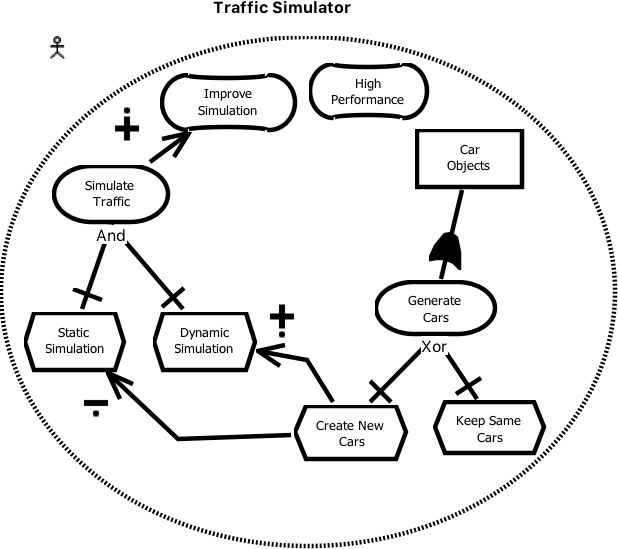
\includegraphics[width=0.5\textwidth]{img/Example1}
\caption{Partial GRL Model of Traffic Simulator Example %(\todo{Marc}{Sepideh}{Turn into vector image, turn ``Dynamic simulation'' and ``Static Simulation'' into goals, turn ``Simulate'' into softgoal, add some resource}}
\label{fig:example-small}
\end{figure} %SG: I changed the figure a bit so that we won't need to change Figure 10. Let me know if you still want to change them according to the above.

\begin{figure*}[ht]
\centering
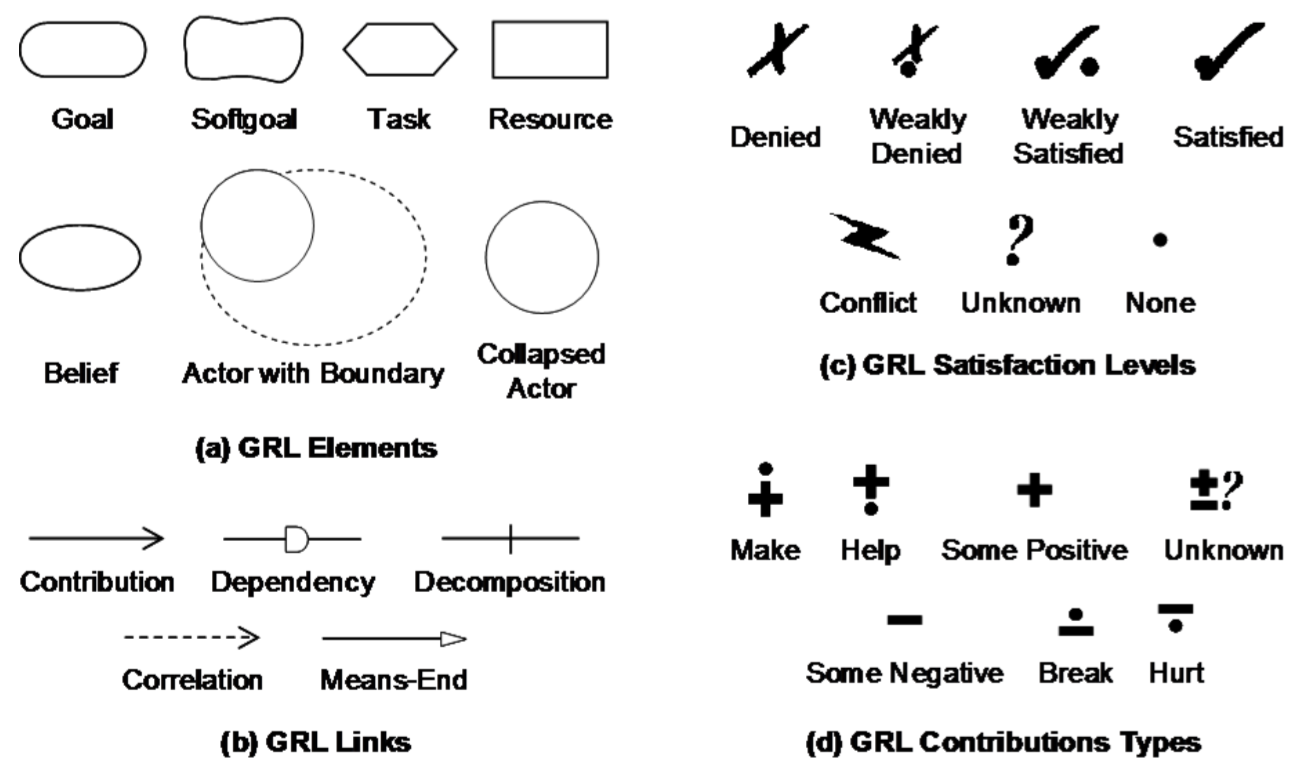
\includegraphics[scale=0.6]{img/grl_legend}
\caption{Basic elements and relationships of GRL}
\label{fig:grl_legend}
\end{figure*}

Figure~\ref{fig:example-small} illustrates a partial GRL diagram from the traffic simulator design exercise (the full figure is shown in Figure~\ref{fig:transcripts:grl} and will be discussed in Section~\ref{sect:gmas}). An actor (
\includegraphics[scale=1]{img/actor}) represents a stakeholder of a system or the system itself (\texttt{Traffic Tycoon}, Figure~\ref{fig:example-small}). Actors are holders of intentions; they are the active entities in the system or its environment who want goals to be achieved, tasks to be performed, resources to be available, and softgoals to be satisfied. Softgoals (
\includegraphics[scale=1]{img/softgoal}) differentiate themselves from goals (
\includegraphics[scale=1]{img/goal}) in that there is no clear, objective measure of satisfaction for a softgoal whereas a goal is quantifiable, often in a binary way. Softgoals (e.g. \texttt{Show Simulation}) are often related to non-functional requirements, whereas goals (such as  \texttt{Generate cars}) are related to functional requirements. Tasks (
\includegraphics[scale=1]{img/task}) represent solutions to (or operationalizations of) goals and softgoals. In Figure~\ref{fig:example-small}, some of the tasks are  \texttt{Create new cars} and \texttt{Keep same cars}. In order to be achieved or completed, softgoals, goals, and tasks may require resources (
\includegraphics[scale=1]{img/resource}) to be available (e.g., \texttt{External Library}).

Different links connect the elements in a GRL model. AND, IOR (Inclusive OR), and XOR (eXclusive OR) decomposition links (
\includegraphics[scale=1]{img/decomposition}) allow an element to be decomposed into sub-elements. In Figure~\ref{fig:example-small}, the goal \texttt{Generate cars} is XOR-decomposed to the tasks \texttt{Create new cars} and \texttt{Keep same cars}. Contribution links (
\includegraphics[scale=1]{img/contribution}) indicate desired impacts of one element on another element. A contribution link has a qualitative contribution type or a quantitative contribution. Task  \texttt{Create new cars} has a \emph{help} qualitative contribution to the task \texttt{Dynamic Simulation}. Dependency links (
\includegraphics[scale=1]{img/dependency}) model relationships between actors. The goal \texttt{Generate Cars} depends on the goal \texttt{Value Has Changed}. %SG: I added it to the model but we can also remove it altogether. 
%\todo{Marc}{Sepideh}{Shall we add a dependency relation as well? They don't play a big role in our work..}

GRL is based on $i*$~\cite{Yu:1997:TMR:827255.827807} and the NFR Framework~\cite{chung2012non}, but it is not as restrictive as $i*$. Intentional elements and links can be more freely combined, the notion of agents is replaced with the more general notion of actors, i.e., stakeholders, and a task does not necessarily have to be an activity performed by an actor, but may also describe properties of a solution. GRL has a well-defined syntax and semantics. Furthermore, GRL provides support for providing a scalable and consistent representation of multiple views/diagrams of the same goal model (see~\cite[Ch.2]{Ghanavati2013} for more details). GRL is also linked to Use Case Maps via URNLink ((
\includegraphics[scale=1]{img/urnlink}) which provides traceability between concepts and instances of the goal model and behavioral design models. Multiple views and traceability links are a good fit with our current research: we aim to add traceability links between intentional elements and their underlying arguments. 

GRL has six evaluation algorithms which are semi-automated and allow the analysis of alternatives and design decisions by calculating the satisfaction value of the intentional elements across multiple diagrams quantitatively, qualitatively or in a hybrid way. The satisfaction values from intentional elements in GRL can also be propagated to the elements of Use Case Maps.  jUCMNav, GRL tool-support, also allows for adding new GRL evaluation algorithms~\cite{jUCMNav}. GRL also has the capability to be extended through metadata, links, and external OCL constraints. This allows GRL to be used in many domains without the need to change the whole modeling language. This feature also helps us apply our argumentation to other domains such as compliance, which we explain in more detail in Section~\ref{sect:goalmodeling:openissues}.

The GRL model in Figure~\ref{fig:example-small} shows the softgoals, goals, tasks and the relationship between the different intentional elements in the model. However, the rationales and arguments behind certain intentional elements are not shown in the GRL model. Some of the questions that might be interesting to know about are the following:

\begin{itemize}
	\item Why does actor \texttt{Traffic Tycoon} have only a single softgoal \texttt{Show Simulation}? Why is this, for instance, not connected to goal \texttt{Simulate}? %SG: I changed this question but let me know if you want to change them back and then change the graph.
	\item What does \texttt{Keep same cars} mean?
	\item Why does task \texttt{Keep same cars} contribute positively to \texttt{Static simulation} and negatively to \texttt{Dynamic simulation}?
	\item Why does \texttt{Generate Cars} XOR-decompose into two tasks?
\end{itemize}

These are the type of the questions that we cannot answer by just looking at GRL models. The model in Figure~\ref{fig:example-small} does not contain information about discussions that lead to the resulting model, such as various clarification steps for the naming, or alternatives that have been considered for the relationships. In this article we aim to address this shortcoming.

\subsection{Argument Scheme for Practical Reasoning (PRAS)}
\label{sect:background:pras}

Reasoning about which goals to pursue and actions to take is often referred to as \emph{practical reasoning}, and has been studied extensively in philosophy (e.g. \cite{Raz1978-RAZPR,walton1990}) and artificial intelligence \cite{bratman1987,atkinson2007}. One approach is to capture practical reasoning using arguments schemes and critical questions~\cite{walton1990}. Applying an argument schemes results in an argument in favor of, for example, taking an action. This argument can, then, be tested with critical questions about, for instance, whether the action is possible given the situation. A negative answer to such a question leads to a counterargument to the original argument for the action. 

Atkinson et al.~\cite{atkinson2007} develop an argument scheme for practical reasoning, which they call the \emph{Practical Reasoning Argument Scheme} (PRAS). This argument scheme is as follows\footnote{The original argument schemes uses slightly different terminology: we have replaced \emph{value} with \emph{softgoal}. Our results do not depend on these adjustments, but they make the relation between PRAS and GRL more clear.}:

\begin{itemize}
\item[] We have goal $G$,
\item[] Doing action $A$ realizes to goal $G$,
\item[] Which will contribute positively to the softgoal $S$
\item[] \textit{Therefore} 
\item[] We should perform action $A$
\end{itemize}

The capital letters $G$, $A$, and $S$ are variables, which can be instantiated with concrete goals, actions, and softgoals. Once instantiated, we obtain an argument. We can for instance instantiate the argument scheme above with the elements of Figure~\ref{fig:example-small} as follows: %SG: Need to update the example.
\begin{itemize}
\item[] We have goal \texttt{Static simulation},
\item[] Doing action \texttt{Keep same cars} realizes goal \texttt{Static simulation}, 
\item[] Which contribute positively to the softgoal \texttt{Simulate} 
\item[] \textit{Therefore} 
\item[] We should perform action \texttt{Keep same cars}.
\end{itemize}

Atkinson \emph{et al.}~\cite{atkinson2007} define a set of critical questions that point to typical ways in which a practical argument can be criticized by, for example, questioning the validity of the elements in the scheme or the connections between the elements. Some examples of critical questions are as follows.

\begin{enumerate}
\item Will the action realize the desired goal?
\item Are there alternative ways of realizing the same goal?
\item Are there alternative ways of contributing to the same softgoal?
\item Does performing the action contribute negatively to some other softgoal?
\item Is the action possible?
\item Can the desired goal be realized?
\item Is the softgoal indeed a legitimate softgoal?
\end{enumerate}

These critical questions can point to new arguments that might counter the original argument. Take, for example, critical question 1: if we find that  \texttt{Keep same cars} actually does not realize goal \texttt{Static Simulation}, we can form a counter-argument. %SG:placeholder for the examples. 

Another way to elaborate an argument for an action is to suggest an alternative action that realizes the same goal (question 2) or an alternative goal that contributes to the same softgoal (question 3). For example,  can argue that another goal \texttt{Semi-dynamic Simulation} also realizes the softgoal \texttt{Simulate}.
\todo{Marc}{Sepideh}{Do you think our example is good? I think it is confusing. Perhaps we should just create an artificial example here, loosely based on the traffic simulator but where the model makes sense to the reader. Now the tasks are all a bit vague and I think nobody knows what they actually mean.}

In argumentation, counterarguments are said to \emph{attack} the original arguments (and sometimes vice versa). In the work of Atkinson et al.~\cite{atkinson2007}, arguments and their attacks are captured as an \emph{argumentation framework} of arguments and attack relations as introduced by Dung~\cite{Dung1995}. Given an argumentation framework, once can compute very precisely which arguments are accepted and which are rejected. 

\subsection{Combining PRAS and GRL}
\label{sect:background:pras:motivation}

The usefulness of argument schemes, and PRAS in particular, for the analysis of practical reasoning situations has been shown in different areas such as e-democracy~\cite{cartwright2009IS}, law~\cite{atkinson2005legal}, planning \cite{medellin2013planning} and choosing between safety critical actions \cite{tolchinsky2012deliberation}. In this article, we aim at capturing the stakeholder's discussions as formal argumentation based on PRAS to decide whether intentional elements and their relationships are shown in the resulting goal model. This approach provides a rationalization to the elements of the goal model in terms of underlying arguments, and furthermore, it helps understanding why certain other elements have been rejected.

Argumentation schemes and their associated critical questions are very well suited for modeling discussions about a goal model: as Murukannaiah et al.~\cite{murukannaiah2015} have shown, they can guide users in systematically deriving conclusions and making assumptions explicit. This can also be seen from the obvious similarities between PRAS (actions, goals, values) and GRL (tasks, goals, softgoals) in the example above.

However, there are also some differences between PRAS and GRL. Not all elements and relationships of GRL fit into PRAS. For instance, PRAS does not have a notion of ``resource'', and many of the relationships of GRL do not occur in PRAS. Furthermore, it is not directly clear whether the critical questions as proposed by Atkinson can actually apply to GRL. Therefore, we develop our own set of argument schemes and critical questions in Section~\ref{sect:gmas} by analyzing transcripts of discussions about the traffic simulator. Before doing so, we give an overview of our framework in the next section.